\documentclass[runningheads]{llncs}

\usepackage{cite}
\usepackage{amsmath,amssymb,amsfonts}
\usepackage{algorithmic}
\usepackage{graphicx}
\usepackage{textcomp}
\usepackage{xcolor}
\usepackage{booktabs}
\usepackage{multirow}
\usepackage{url}

\begin{document}

\title{PQC-FL-Health: Post-Quantum Federated Learning\\
for Privacy-Preserving Healthcare Analytics}

\author{Anonymous Author}
\authorrunning{Anonymous Author}
\institute{Anonymous Institution}
\titlerunning{PQC-FL-Health: Post-Quantum Federated Learning}

\maketitle

\begin{abstract}
Federated learning (FL) allows hospitals to collaboratively train
machine learning models without transferring raw patient data.
Most existing FL deployments use classical cryptographic schemes such
as RSA and HMAC, which are vulnerable to harvest-now-decrypt-later
attacks by quantum-capable adversaries.
We present \textbf{PQC-FL-Health}, a three-layer security framework
for federated healthcare analytics that replaces classical primitives
with NIST-standardised post-quantum cryptography (PQC):
(1)~\textbf{ML-KEM-768} (CRYSTALS-Kyber) for quantum-safe key
encapsulation, (2)~\textbf{ML-DSA-65} (CRYSTALS-Dilithium) for
authenticated gradient updates, and (3)~\textbf{Gaussian differential
privacy (DP)} to guard against aggregator-side patient-data inference.
We evaluate the system on a node-specialised five-hospital federation
in which each hospital holds its own disease domain
(Pima diabetes, Cleveland heart disease, WDBC breast cancer),
and on a homogeneous single-disease scenario with non-IID
glucose-quartile partitioning as the primary FL evaluation.
Over five random seeds and 50 communication rounds, PQC-FL-Health
achieves global AUC $0.888 \pm 0.005$ on the heterogeneous
federation, with per-disease AUC of $0.798$ (diabetes),
$0.845$ (heart disease), and $0.996$ (breast cancer).
PQC operations complete in under 1\,ms at all three NIST security
levels and run \textbf{1.6$\times$ faster} end-to-end than RSA-4096
(64\,ms vs.\ 103\,ms per round), despite adding 31.1\,KB of
cryptographic overhead per round.
ML-DSA signature verification detects 100\% of tampered-signature
attacks; a gradient-norm filter catches all tested scaled-gradient
poisoning attempts.
At $\varepsilon = 10$, differential privacy costs 15\% AUC on the
homogeneous federation; budgets at or below $\varepsilon = 1$ cause
both severe degradation and high cross-seed variance, confirming that
tight DP is not viable for 1531-parameter models.
Code and datasets are available upon acceptance.
\end{abstract}

\keywords{federated learning \and post-quantum cryptography \and
differential privacy \and Byzantine robustness \and ML-KEM \and
ML-DSA \and healthcare AI}

%==================================================================
\section{Introduction}
\label{sec:intro}

Healthcare institutions generate large volumes of sensitive patient
data that are distributed across hospitals, clinics, and research
centres.
Federated learning (FL)~\cite{mcmahan2017} lets these institutions
jointly train shared models without centralising raw records,
preserving patient privacy by design.
However, FL deployments in production healthcare systems face two
threats that are rarely addressed together.

\textbf{The quantum threat.}
Classical public-key cryptography, including RSA, Diffie-Hellman, and
ECDSA, underpins the secure channels over which FL updates travel.
Shor's algorithm~\cite{shor1994} can break these schemes in polynomial
time on a sufficiently powerful quantum computer.
More immediately, adversaries can record encrypted model updates today
and decrypt them once quantum hardware matures, exposing both the
model and the patient data used to train it.
NIST has responded by standardising ML-KEM (FIPS~203)~\cite{nistfips203}
and ML-DSA (FIPS~204)~\cite{nistfips204}, two lattice-based schemes
designed to resist quantum attacks.

\textbf{The federated attack surface.}
Even with a secure channel, FL aggregation is vulnerable to Byzantine
nodes that inject malicious gradient updates~\cite{blanchard2017}, and
to honest-but-curious aggregators that infer patient attributes from
received updates~\cite{geiping2020}.
Differential privacy (DP)~\cite{dwork2006} is the standard defence
against aggregator inference, but its interaction with FL convergence
under non-IID healthcare data is not well characterised empirically.

\textbf{Contributions.} This paper makes the following contributions:
\begin{itemize}
  \item We design and implement \textbf{PQC-FL-Health}, a federated
    learning system for healthcare that, to the best of our knowledge,
    is the first to simultaneously provide quantum-safe channel security
    (ML-KEM-768), authenticated updates (ML-DSA-65), Byzantine
    robustness via signature verification and gradient-norm filtering,
    and differential privacy via the Gaussian mechanism with empirical
    benchmarks against RSA-4096.

  \item We benchmark all three NIST post-quantum security levels
    (ML-KEM-512/768/1024 paired with ML-DSA-44/65/87) on a realistic
    12\,KB model-delta payload, reporting latency, bandwidth overhead,
    and convergence quality.

  \item We evaluate two clinically motivated federation scenarios:
    a node-specialised five-hospital federation spanning three disease
    domains with local-vs-federated comparison, and a homogeneous
    five-clinic federation for diabetes prediction under extreme
    non-IID glucose-quartile partitioning.

  \item We quantify the privacy-utility tradeoff for DP in small-model
    FL, showing that $\varepsilon = 10$ costs $\approx$15\% AUC
    (0.753$\to$0.639), while $\varepsilon \le 1$ yields unpredictable
    variance on a 1531-parameter model, providing a practical baseline
    for future work on DP-compatible architectures.
\end{itemize}

Section~\ref{sec:related} reviews related work.
Section~\ref{sec:system} describes the system architecture.
Section~\ref{sec:setup} covers the experimental setup.
Section~\ref{sec:results} presents results.
Section~\ref{sec:conclusion} concludes.

%==================================================================
\section{Related Work}
\label{sec:related}

FedAvg~\cite{mcmahan2017} remains the dominant FL aggregation rule;
Li~et~al.~\cite{li2020federated} survey its challenges including
non-IID data~\cite{zhao2018} and systems heterogeneity.
FL in medical imaging~\cite{rieke2020} motivates privacy-preserving
aggregation without data centralisation.
PQC for FL is nascent: Cheng~et~al.~\cite{cheng2023pqcfl} propose a
PQC communication model for quantum FL;
Huang~et~al.~\cite{huang2024pqcfl} study NIST PQC signatures in FL;
PQS-BFL~\cite{pierson2025pqsbfl} combines PQC with blockchain-based FL;
a 2025 survey~\cite{survey2025flquantum} reviews the FL--quantum
intersection.
On Byzantine robustness, Blanchard~et~al.~\cite{blanchard2017}
introduced Krum; Fang~et~al.~\cite{fang2020} showed adaptive
poisoning can bypass many defences.
On privacy, Abadi~et~al.~\cite{abadi2016} introduced DP-SGD;
Geyer~et~al.~\cite{geyer2017} applied client-level DP to FL.
To the best of our knowledge, no prior work combines ML-KEM key
encapsulation, ML-DSA gradient authentication, Byzantine
defence-in-depth, and Gaussian DP in a single healthcare FL system
with empirical benchmarks against RSA-4096.

%==================================================================
\section{System Design}
\label{sec:system}

\subsection{Architecture Overview}

PQC-FL-Health uses a standard cross-silo FL topology: $N = 5$
hospital nodes communicate with a central aggregation server over
simulated secure channels.
Each node holds a private local dataset and a local model copy.
In each communication round, nodes: (1) receive the current global
weights from the server, (2) train locally for $E = 5$ epochs,
(3) compute a weight delta $\Delta_i = w_i^{\text{new}} - w^{\text{global}}$,
(4) optionally apply DP noise, (5) encrypt and sign $\Delta_i$ using
PQC primitives, and (6) transmit the bundle.
The server verifies each bundle, aggregates accepted updates with
FedAvg, and broadcasts the new global weights.

\subsection{Layer 1: Quantum-Safe Confidentiality (ML-KEM-768)}

The server generates a long-term ML-KEM-768 keypair and publishes its
public key.
Before sending an update, each node encapsulates a shared secret:
\begin{equation}
  (\text{ct}, K) \leftarrow \text{ML-KEM.Encaps}(\text{pk}_{\text{server}})
\end{equation}
The shared secret $K$ is expanded via HKDF-SHA256 to a 256-bit
AES-GCM key, which encrypts the serialised gradient delta:
\begin{equation}
  c \leftarrow \text{AES-256-GCM.Enc}(K,\ \Delta_i)
\end{equation}
The transmitted bundle contains $(\text{ct},\ c,\ \text{nonce})$.
The server decapsulates $\text{ct}$ to recover $K$ and decrypts $c$.
ML-KEM-768 achieves NIST security level~3 (AES-192 equivalent) with a
ciphertext of 1088\,bytes and average encapsulation latency under
0.3\,ms in our environment.

\subsection{Layer 2: Authenticated Updates (ML-DSA-65)}

Each node holds a long-term ML-DSA-65 signing keypair; the server
maintains a registry of node public keys established at setup time
and not retransmitted each round.
After encryption, the node signs the concatenation of the KEM
ciphertext and AES ciphertext:
\begin{equation}
  \sigma \leftarrow \text{ML-DSA.Sign}(\text{sk}_i,\ \text{ct} \| c)
\end{equation}
The server verifies $\sigma$ before accepting any update.
A node that sends a tampered or forged signature is immediately
rejected and its update discarded.
ML-DSA-65 signatures are 3309\,bytes with verification latency under
0.3\,ms, providing NIST security level~3 authentication.

\subsection{Layer 3: Aggregator-Side Privacy (Differential Privacy)}

To protect against an honest-but-curious aggregator that may infer
patient attributes from gradient updates, we apply the Gaussian
mechanism~\cite{dwork2006} at the node level.
Each node clips its delta to $\ell_2$ sensitivity $S = 0.1$ and adds
calibrated Gaussian noise:
\begin{equation}
  \tilde{\Delta}_i = \text{clip}_{S}(\Delta_i)
    + \mathcal{N}(0,\ \sigma^2 \mathbf{I}), \quad
  \sigma = \frac{S\,\sqrt{2\ln(1.25/\delta)}}{\varepsilon}
\end{equation}
with $\delta = 10^{-5}$ fixed and $\varepsilon$ as the privacy budget.
DP noise is added before PQC encryption, so the server never observes
the original gradient.
Privacy loss is tracked across rounds using R\'{e}nyi differential
privacy (RDP) composition~\cite{mironov2017rdp}, which yields tighter
cumulative bounds than naive linear composition; at 50 rounds and
$\varepsilon_{\text{per-round}}=10$, the RDP accountant gives
$\varepsilon_{\text{cumul}}=181.7$ vs.\ $500$ under naive addition.

\subsection{Byzantine Defence}

Our defence operates at two levels.
First, ML-DSA signature verification (Layer~2) immediately rejects
any bundle that fails cryptographic authentication, covering
tampered-signature attacks with 100\% detection.
Second, after decryption, the server optionally applies a
gradient-norm anomaly filter:
\begin{equation}
  \text{reject node } i \text{ if } \|\Delta_i\|_2 > 3 \cdot \text{median}_j\|\Delta_j\|_2
\end{equation}
This catches gradient-scaling attacks where a rogue node sends a
correctly signed but amplified delta.

\subsection{Aggregation}

Accepted updates are aggregated with FedAvg weighted by local
dataset size:
\begin{equation}
  w^{\text{new}} = w^{\text{global}} +
    \sum_{i \in \mathcal{A}} \frac{n_i}{\sum_{j\in\mathcal{A}} n_j}\,\Delta_i
\end{equation}
where $\mathcal{A}$ is the set of accepted nodes and $n_i$ is node
$i$'s training set size.

%==================================================================
\section{Experimental Setup}
\label{sec:setup}

\subsection{Datasets and Non-IID Partitioning}

We evaluate on two federation scenarios.

\textbf{Homogeneous federation (FL convergence benchmark).}
All five nodes hold disjoint shards of the Pima Indians Diabetes
dataset~\cite{smith1988} (768 samples, 8 features, 34.9\% positive),
partitioned \emph{non-IID} by ascending glucose level (feature~2).
This produces extreme label skew: node~0 (low-glucose patients)
has 8.1\% positive rate, while node~4 (high-glucose referral
centre) has 73.2\% positive rate, a $9\times$ ratio.
This is a methodologically clean cross-silo FL benchmark: all nodes
share the same prediction task and label semantics.

\textbf{Heterogeneous federation (system validation).}
Five simulated hospitals each specialise in a single disease domain:
nodes~0--1 hold independent shards of the Pima Indians Diabetes
dataset~\cite{smith1988} (8 features, $\sim$205 training samples each);
node~2 holds the Cleveland Heart Disease
dataset~\cite{detrano1989} (13 features, 238 training samples, 46\%
positive); node~3 holds the Wisconsin Diagnostic Breast Cancer
(WDBC) dataset~\cite{street1993} (30 features, 456 training samples,
37\% positive); node~4 holds a third Pima shard with Gaussian
feature noise ($\sigma=0.1$) simulating a lower-quality data source.
All features are zero-padded to 30 dimensions.
Each hospital normalises its own features independently.
This scenario tests whether PQC-FL-Health operates correctly under
data heterogeneity; a local-vs.-federated comparison
(Section~\ref{sec:results}) quantifies the benefit and cost of
cross-disease gradient sharing.

\subsection{Model and Training}

Each hospital trains a fully connected multi-layer perceptron (MLP)
with three layers ($30 \to 64 \to 32 \to 1$, ReLU activations,
sigmoid output, 1531 parameters) for $E = 5$ local epochs per round
using SGD with learning rate $\eta = 0.01$.
An MLP is appropriate here given that all three datasets are tabular.
Binary cross-entropy loss is used throughout with mini-batches
of size 32.

\subsection{Evaluation Protocol}

We run 50 communication rounds per seed across five random seeds
(42, 123, 456, 789, 1337) and report mean $\pm$ standard deviation.
The global test set is the union of all hospital test sets; for the
heterogeneous scenario we also report per-disease AUC separately.
The primary metric is AUROC (AUC); we also report sensitivity,
specificity, F1, and accuracy.

Cryptographic benchmarks use 20 iterations per configuration on a
12\,KB payload representative of a model delta.
All experiments run on Python~3.12 under Ubuntu WSL2 (Linux~6.6,
no GPU) on an AMD Ryzen 7 7435HS CPU, using liboqs~0.15.0 via
liboqs-python~0.14.1.

%==================================================================
\section{Results}
\label{sec:results}

\subsection{FL Convergence and Local Baseline}

Fig.~\ref{fig:convergence} shows convergence curves for both
federation scenarios across five seeds.

\textbf{Homogeneous Pima-only federation (primary).}
Final AUC is $0.787 \pm 0.019$ (Table~\ref{tab:convergence}).
The extreme non-IID skew---nodes spanning 8--73\% positive
rate---forces FedAvg to reconcile fundamentally different local
optima, explaining the residual variance and the gap relative to
a balanced dataset.

\textbf{Heterogeneous federation (system stress-test).}
Global AUC rises from $0.472 \pm 0.082$ (round~1) to
$\mathbf{0.888 \pm 0.005}$ (round~50).
Fig.~\ref{fig:convergence} (left) also shows per-disease convergence:
breast cancer (WDBC) saturates early at AUC~$0.996 \pm 0.002$,
while diabetes and heart disease converge more gradually to
AUC~$0.798 \pm 0.013$ and $0.845 \pm 0.011$, respectively
(Table~\ref{tab:convergence}).

To determine whether cross-disease gradient sharing provides utility,
we compare against a \emph{local baseline} in which each hospital
trains in complete isolation for the same total gradient steps
($50~\text{rounds} \times 5~\text{local epochs}$).
Table~\ref{tab:local_vs_fed} shows the results.
Cancer (WDBC, $n{=}456$ training) is self-sufficient: local
$0.995 \pm 0.003$ vs.\ federated $0.996 \pm 0.002$
($\Delta = +0.001$).
Heart disease incurs a \textbf{gradient-dilution penalty}: federated
AUC ($0.845 \pm 0.011$) is 6.5 points below local ($0.910 \pm 0.030$)
because WDBC gradients from semantically disjoint features interfere
with Cleveland's 13-dimensional signal.
Diabetes shows the same mean ($0.799$ vs.\ $0.798$) but federation
reduces prediction variance \textbf{4.8$\times$}
($\pm0.058 \to \pm0.012$), providing more stable clinical
decision-support for hospitals with only $\sim$200 training samples.

These results reveal an inherent tradeoff in cross-disease
federation: variance stabilisation for data-scarce nodes versus
accuracy degradation from gradient dilution.
Critically, the PQC security layer operates identically in both
regimes; the quantum-safety guarantees are independent of whether
the federation scope is clinically optimal.
Determining appropriate federation scope is a domain decision;
future work should explore multi-task FL architectures (per-disease
output heads) to eliminate gradient interference while preserving
variance reduction.

\begin{figure}[t]
  \centering
  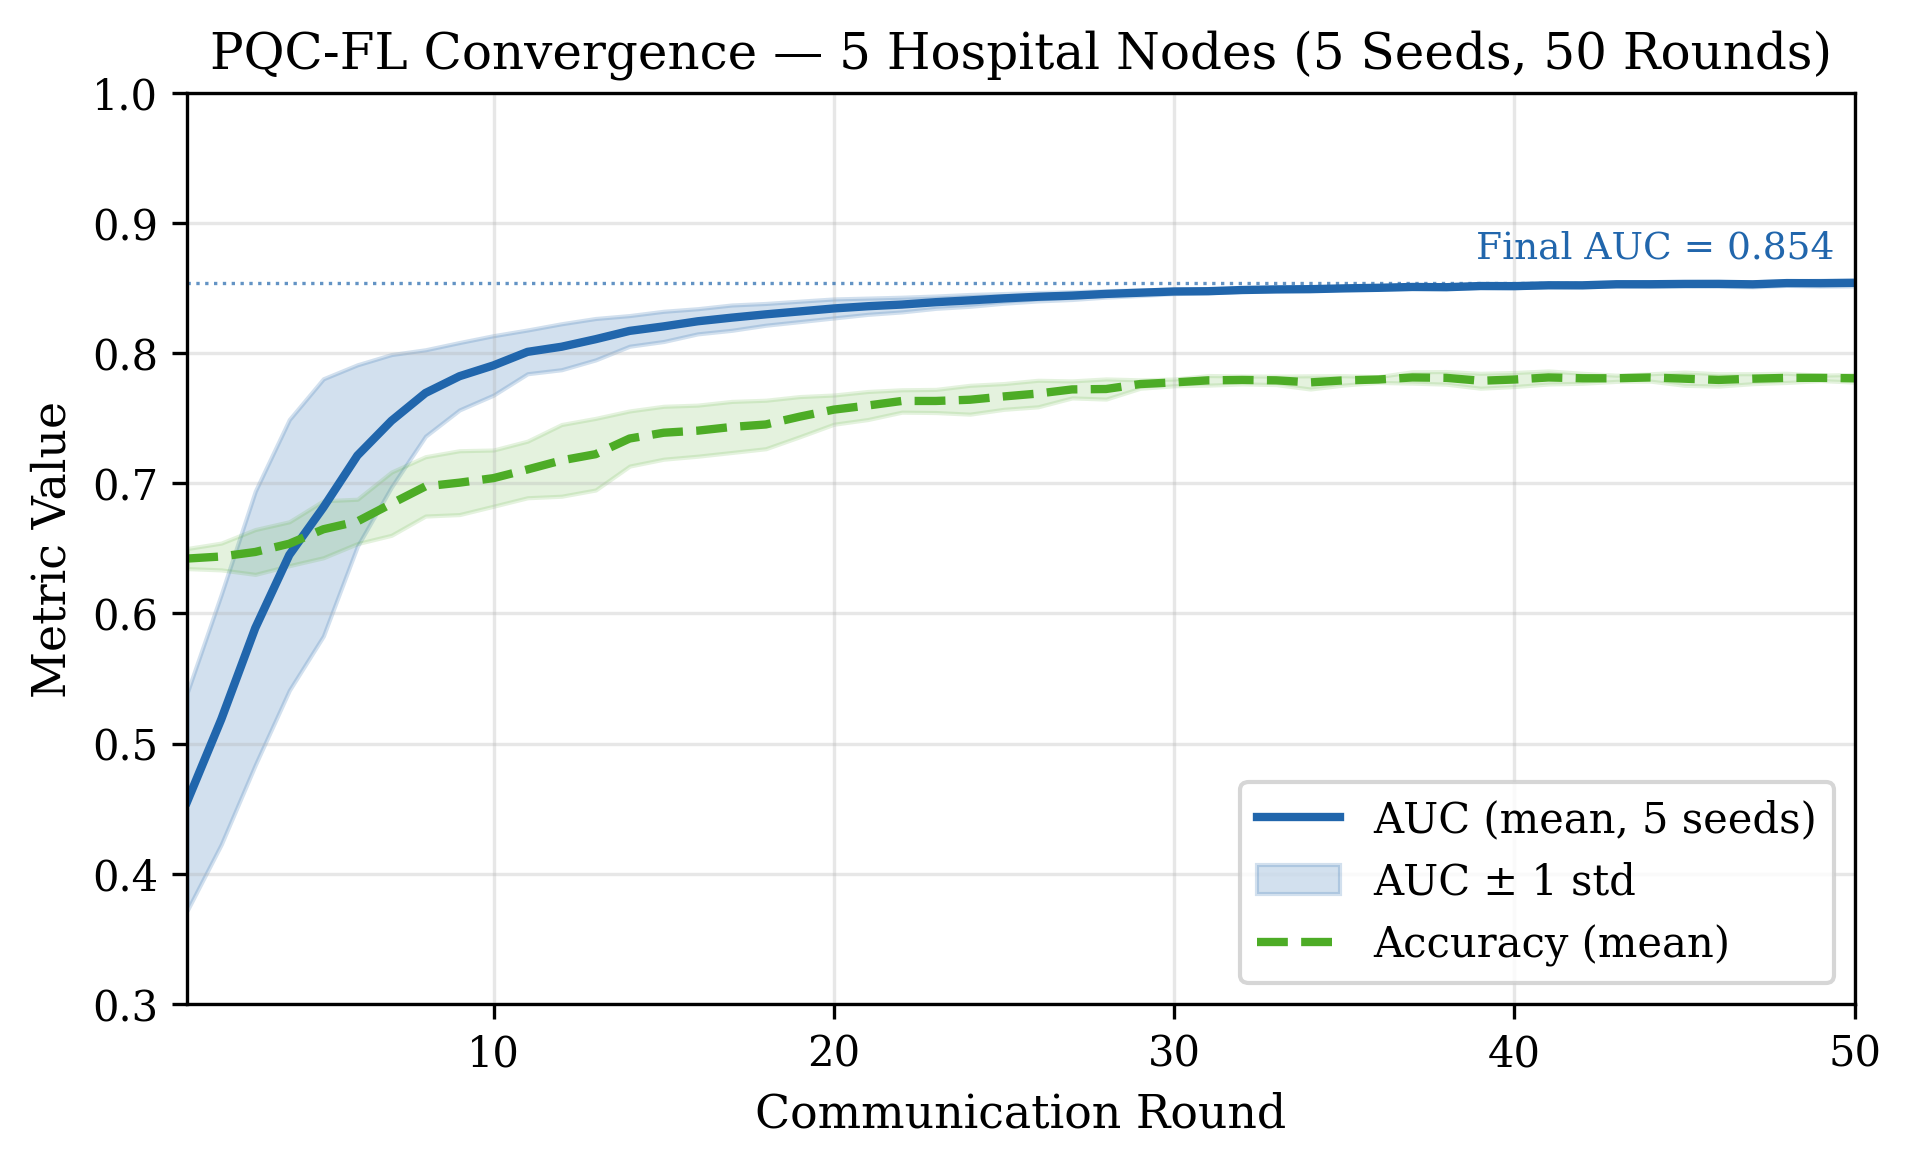
\includegraphics[width=\linewidth]{fig1_convergence.png}
  \caption{FL convergence over 50 rounds across 5 random seeds.
    \textbf{Left:} Heterogeneous federation---each of the 5 hospitals
    specialises in one disease domain.
    Solid line: global AUC $0.888 \pm 0.005$;
    dashed lines show per-disease AUC
    (cancer $0.996$, heart $0.845$, diabetes $0.798$).
    \textbf{Right:} Homogeneous federation (primary)---5 diabetes
    clinics partitioned non-IID by glucose quartile
    (AUC $0.787 \pm 0.019$).
    Shaded bands: $\pm 1$ std across seeds.}
  \label{fig:convergence}
\end{figure}

\begin{table}[t]
  \caption{Final Model Quality (Round 50, 5 Seeds)}
  \label{tab:convergence}
  \centering
  \begin{tabular}{lcc}
    \toprule
    \textbf{Metric} & \textbf{Hetero (global)} & \textbf{Homogeneous (Pima)} \\
    \midrule
    AUC              & $0.888 \pm 0.005$ & $0.787 \pm 0.019$ \\
    AUC --- Diabetes & $0.798 \pm 0.013$ & --- \\
    AUC --- Heart    & $0.845 \pm 0.011$ & --- \\
    AUC --- Cancer   & $0.996 \pm 0.002$ & --- \\
    Sensitivity      & $0.638 \pm 0.021$ & $0.312 \pm 0.067$ \\
    Specificity      & $0.908 \pm 0.009$ & $0.900 \pm 0.033$ \\
    F1 Score         & $0.712 \pm 0.011$ & $0.412 \pm 0.064$ \\
    Accuracy         & $0.807 \pm 0.004$ & $0.696 \pm 0.023$ \\
    \bottomrule
  \end{tabular}
\end{table}

\begin{table}[t]
  \caption{Heterogeneous Federation: Local vs.\ Federated AUC
           (Round 50, 5 Seeds)}
  \label{tab:local_vs_fed}
  \centering
  \begin{tabular}{lccc}
    \toprule
    \textbf{Disease} & \textbf{Local} & \textbf{Federated} & $\boldsymbol{\Delta}$ \textbf{AUC} \\
    \midrule
    Diabetes  & $0.799 \pm 0.058$ & $0.798 \pm 0.012$ & $-0.001$ \\
    Heart     & $0.910 \pm 0.030$ & $0.845 \pm 0.011$ & $-0.065$ \\
    Cancer    & $0.995 \pm 0.003$ & $0.996 \pm 0.002$ & $+0.001$ \\
    \bottomrule
  \end{tabular}
  \\[3pt]
  {\footnotesize Positive $\Delta$ = federation improves on local training.
  Diabetes variance reduction: $\pm0.058 \to \pm0.012$ (4.8$\times$).}
\end{table}

\subsection{PQC vs.\ Classical Cryptography}

Table~\ref{tab:pqcvscls} compares PQC (ML-KEM-768 + ML-DSA-65 +
AES-256-GCM) against the classical baseline (RSA-4096 + HMAC-SHA256 +
AES-256-GCM) over 30 rounds and 5 nodes.
Both schemes reach identical model quality (AUC~0.837), confirming
that replacing classical primitives with PQC does not affect
convergence.

PQC is \textbf{1.6$\times$ faster} per round (64\,ms vs.\ 103\,ms).
This advantage comes primarily from decryption: ML-KEM-768
decapsulation takes 1.41\,ms per round, while RSA-4096 decryption
takes 33.44\,ms, a \textbf{24$\times$ speedup}.
RSA decryption cost scales with key size, whereas lattice-based KEM
decapsulation runs in $O(n \log n)$ polynomial ring arithmetic.
Note that node-side PQC encrypt+sign (0.57\,ms) is modestly slower
than RSA encrypt+HMAC (0.29\,ms); the end-to-end advantage is driven
by server-side decapsulation, which dominates round time.
Fig.~\ref{fig:latency} shows per-round latency traces across all
30 rounds.

\begin{table}[t]
  \caption{PQC vs.\ Classical: 30 Rounds, 5 Nodes}
  \label{tab:pqcvscls}
  \centering
  \begin{tabular}{lrr}
    \toprule
    \textbf{Metric} & \textbf{PQC} & \textbf{Classical} \\
    \midrule
    AUC                      & 0.837 & 0.837 \\
    Avg round time (ms)      & 64    & 103   \\
    Avg enc / node (ms)      & 0.57  & 0.29  \\
    Avg dec / round (ms)     & 1.41  & 33.44 \\
    Total bandwidth (30r)    & 3381\,KB & 2531\,KB \\
    Crypto overhead / round  & 31.1\,KB & 2.8\,KB \\
    \bottomrule
  \end{tabular}
\end{table}

\begin{figure}[t]
  \centering
  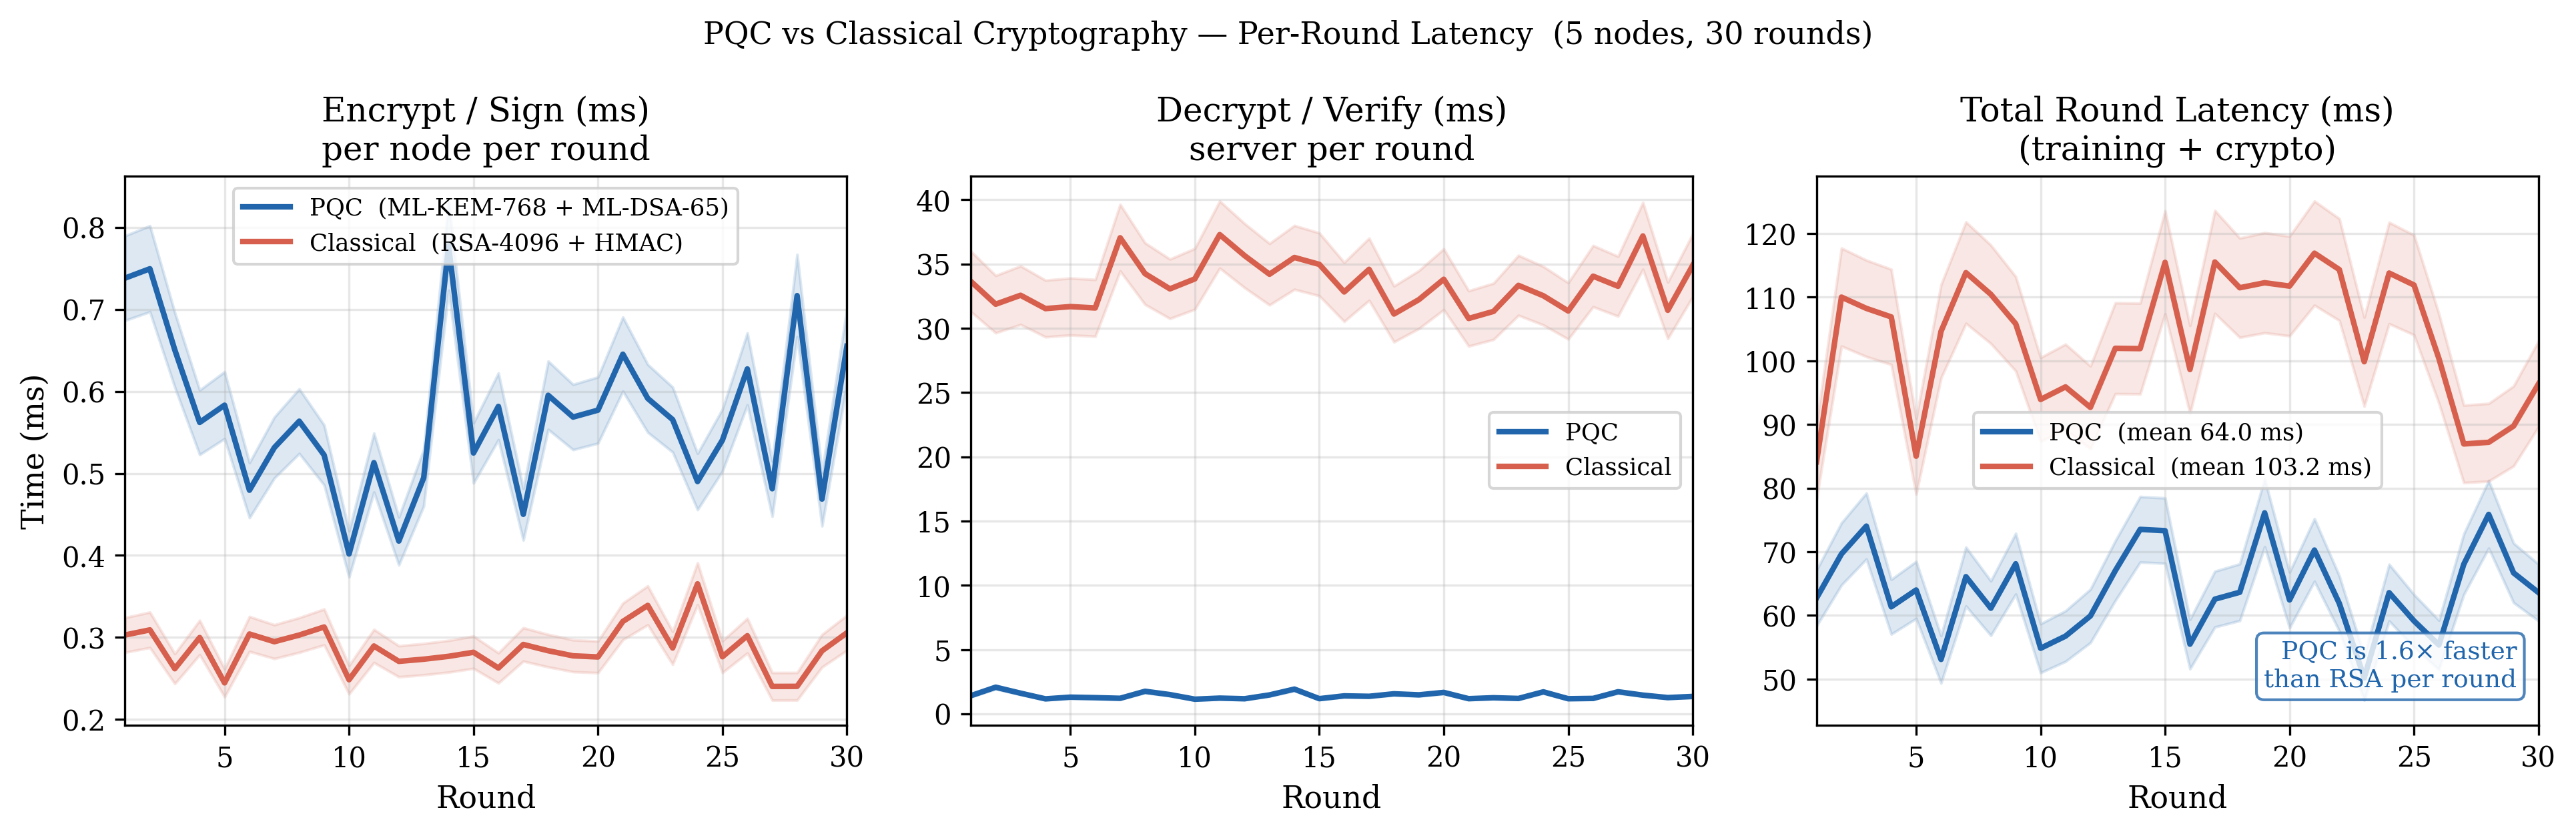
\includegraphics[width=\linewidth]{fig4_latency_breakdown.png}
  \caption{Per-round latency breakdown over 30 rounds (5 nodes).
    \textbf{Left:} Node-side encrypt+sign time per round.
    \textbf{Centre:} Server-side decrypt+verify time per round.
    \textbf{Right:} Total round time (training + cryptography).
    PQC decryption (1.41\,ms) is 24$\times$ faster than RSA-4096
    (33.44\,ms), yielding a 1.6$\times$ end-to-end speedup
    (64\,ms vs.\ 103\,ms).}
  \label{fig:latency}
\end{figure}

\subsection{NIST Security Level Comparison}

Fig.~\ref{fig:seclevels} and Table~\ref{tab:seclevels} benchmark
all three NIST post-quantum security levels on a 12\,KB model-delta
payload (20 iterations each).
Round-trip latency stays below 1\,ms at all levels.
Level~3 (ML-KEM-768 + ML-DSA-65) is slightly faster than Level~1
in our environment (0.713\,ms vs.\ 0.940\,ms), which we attribute
to CPU cache behaviour and the optimisation profile of liboqs~0.15.0.
Cryptographic overhead grows with security level: 4.4\,KB (Level~1),
6.2\,KB (Level~3), 8.6\,KB (Level~5).
For a 12\,KB model delta, even the highest level adds 72\% overhead
in bytes, a modest cost for quantum-safe guarantees.

\begin{table}[t]
  \caption{NIST Security Level Comparison (12\,KB payload, 20 iter.)}
  \label{tab:seclevels}
  \centering
  \resizebox{\linewidth}{!}{%
  \begin{tabular}{lccc}
    \toprule
    \textbf{Metric} & \textbf{Level~1} & \textbf{Level~3} & \textbf{Level~5} \\
    & ML-KEM-512 & ML-KEM-768 & ML-KEM-1024 \\
    & +ML-DSA-44 & +ML-DSA-65 & +ML-DSA-87 \\
    \midrule
    Enc+Sign (ms)       & 0.72 & 0.41 & 0.46 \\
    Dec+Verify (ms)     & 0.22 & 0.31 & 0.31 \\
    Round-trip (ms)     & 0.94 & 0.71 & 0.77 \\
    KEM ciphertext (B)  & 768  & 1088 & 1568 \\
    Signature (B)       & 2420 & 3309 & 4627 \\
    Crypto overhead (KB)& 4.4  & 6.2  & 8.6  \\
    \bottomrule
  \end{tabular}}
\end{table}

\begin{figure}[t]
  \centering
  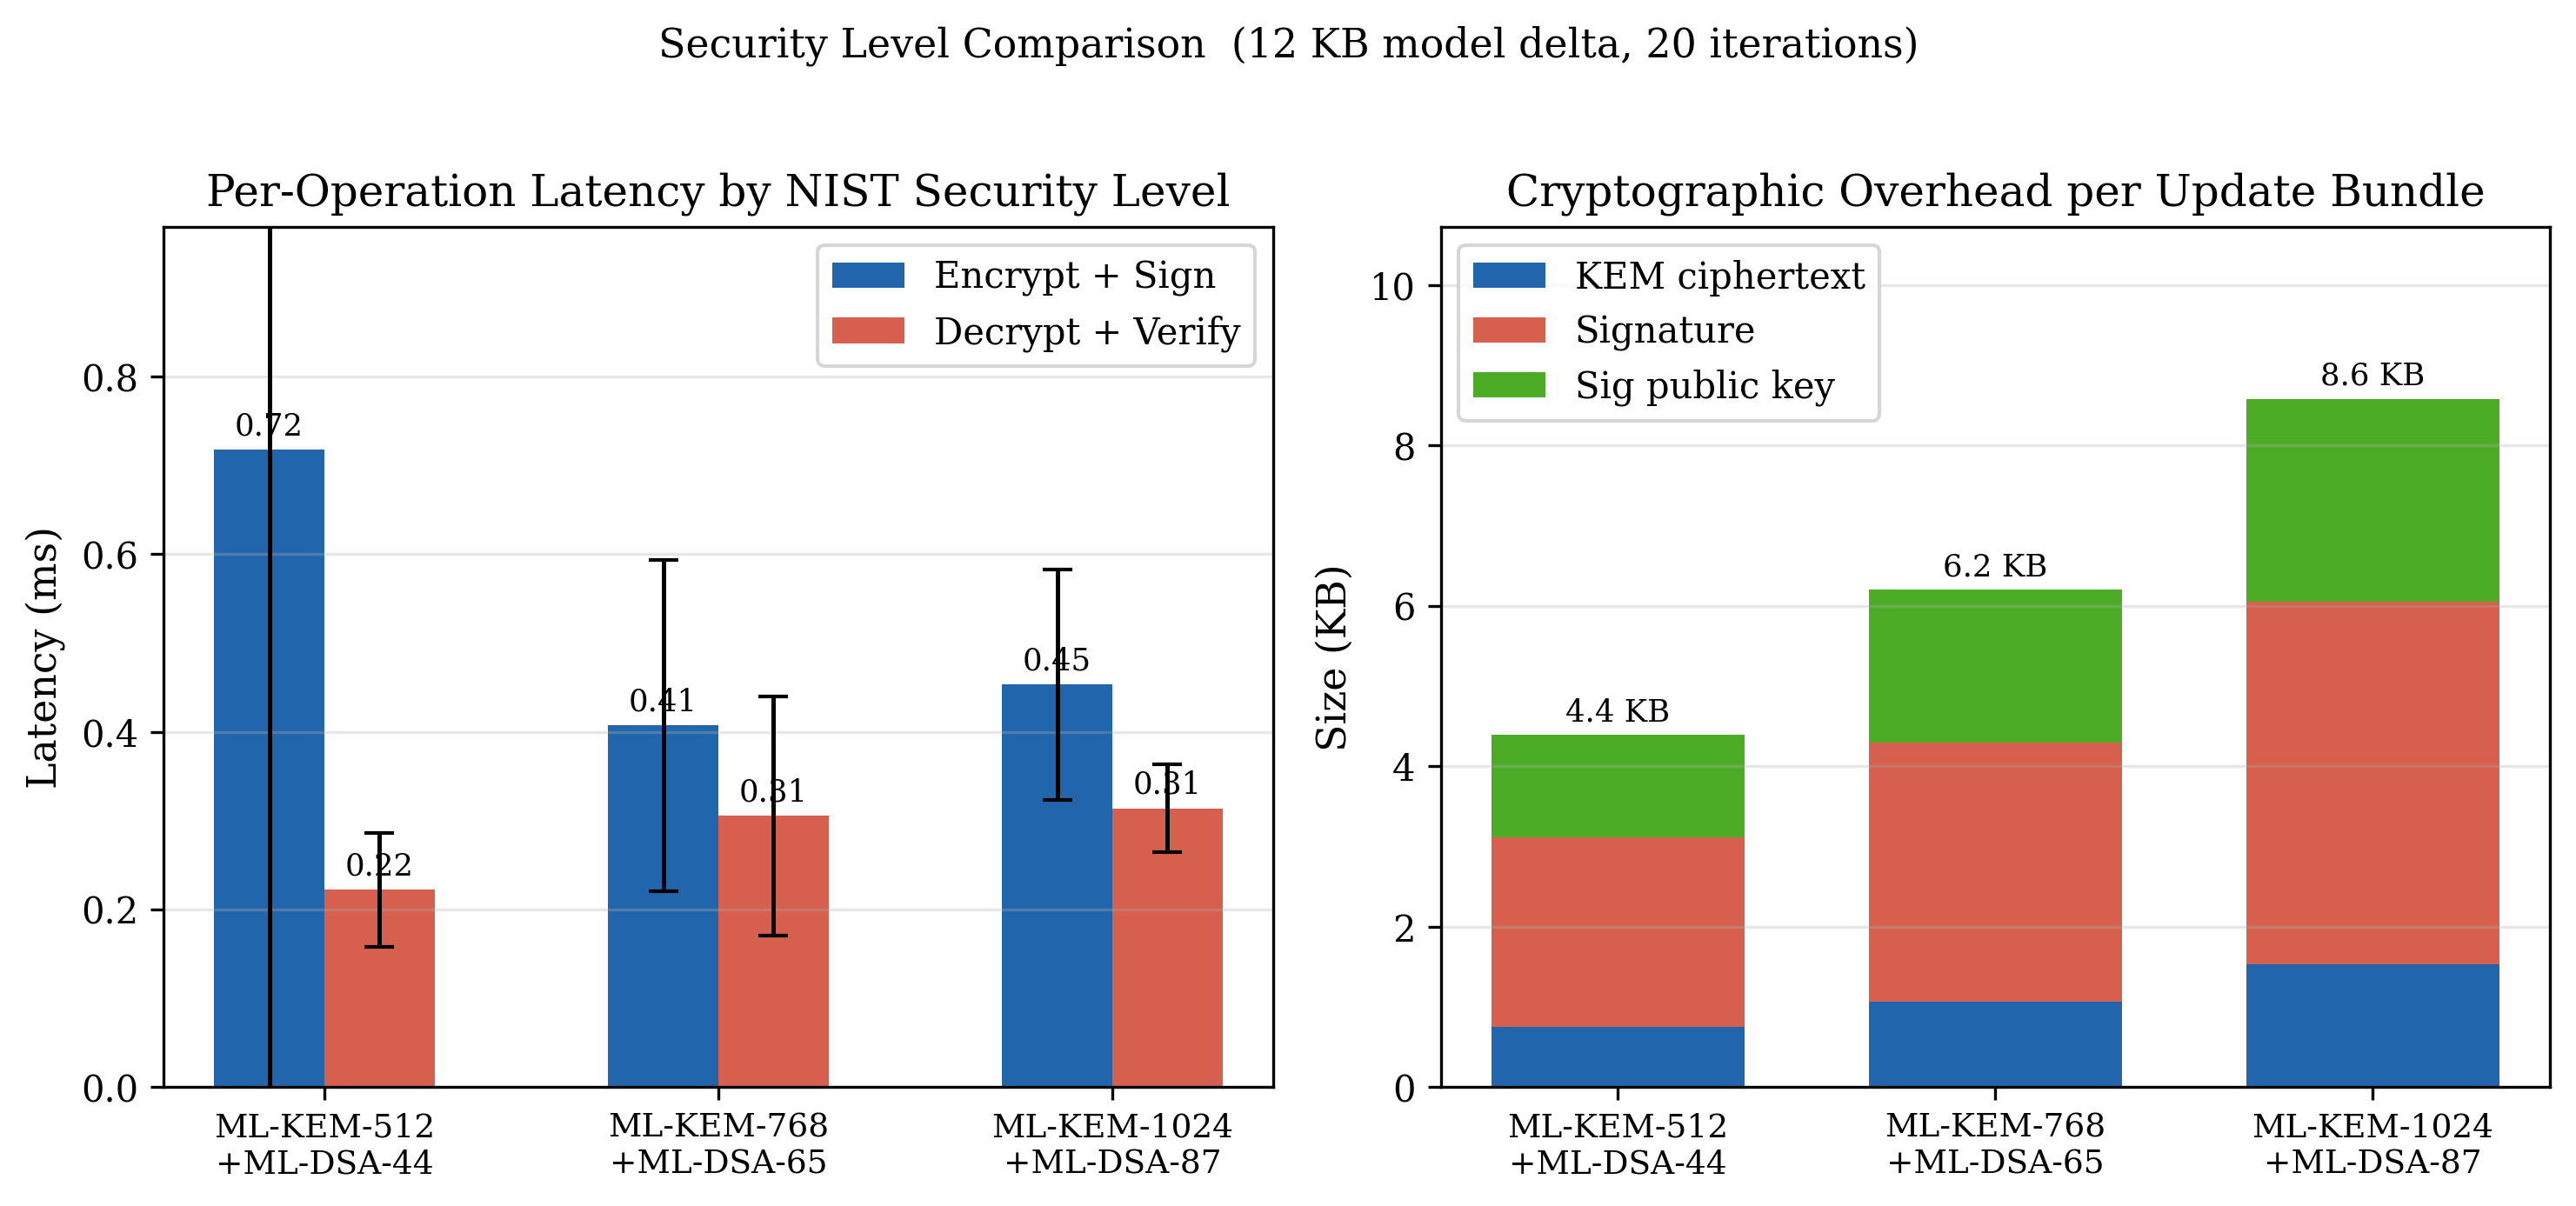
\includegraphics[width=\linewidth]{fig2_security_levels.png}
  \caption{NIST post-quantum security level comparison on a 12\,KB
    model-delta payload (20 iterations each).
    \textbf{Left:} Per-operation latency (mean $\pm$ std).
    All levels complete encrypt+sign and decrypt+verify under 0.8\,ms.
    \textbf{Right:} Cryptographic overhead per update bundle, broken
    down into KEM ciphertext, signature, and signing public key.
    Overhead ranges from 4.4\,KB (Level~1) to 8.6\,KB (Level~5).}
  \label{fig:seclevels}
\end{figure}

\subsection{Byzantine Attack and Defence}

Fig.~\ref{fig:byzantine} shows the two-part Byzantine evaluation
over 20 rounds with node~4 as the rogue node, repeated across
3 random seeds (60 rounds total per attack type).

\textbf{Part A: Tampered Signature Attack.}
The rogue node flips the first 32 bytes of its ML-DSA signature
before transmission.
ML-DSA verification rejects the bundle in \textbf{100\% of rounds
across all 3 seeds (60/60)}.
The global model trains on the remaining four honest nodes and
converges more slowly than the clean baseline, reflecting the lost
data contribution from one hospital shard, but no adversarial
gradient ever enters the global model.

\textbf{Part B: Gradient Poisoning Attack.}
The rogue node sends a correctly signed but 50$\times$-scaled gradient
delta.
Without the norm filter, the poisoned model reaches
AUC~$0.619 \pm 0.114$ at round~20, far below the clean baseline.
With the gradient-norm filter ($3\times$ median threshold), the rogue
node is rejected in \textbf{100\% of rounds across all seeds}, and the
defended model recovers to AUC~$0.865 \pm 0.006$.
The $\Delta = +0.246$ gap between defended and undefended AUC
directly illustrates the value of the second-layer filter.
These results confirm that ML-DSA authentication provides a
cryptographic first line of defence, and the norm filter forms
an effective statistical second line.

\begin{figure}[t]
  \centering
  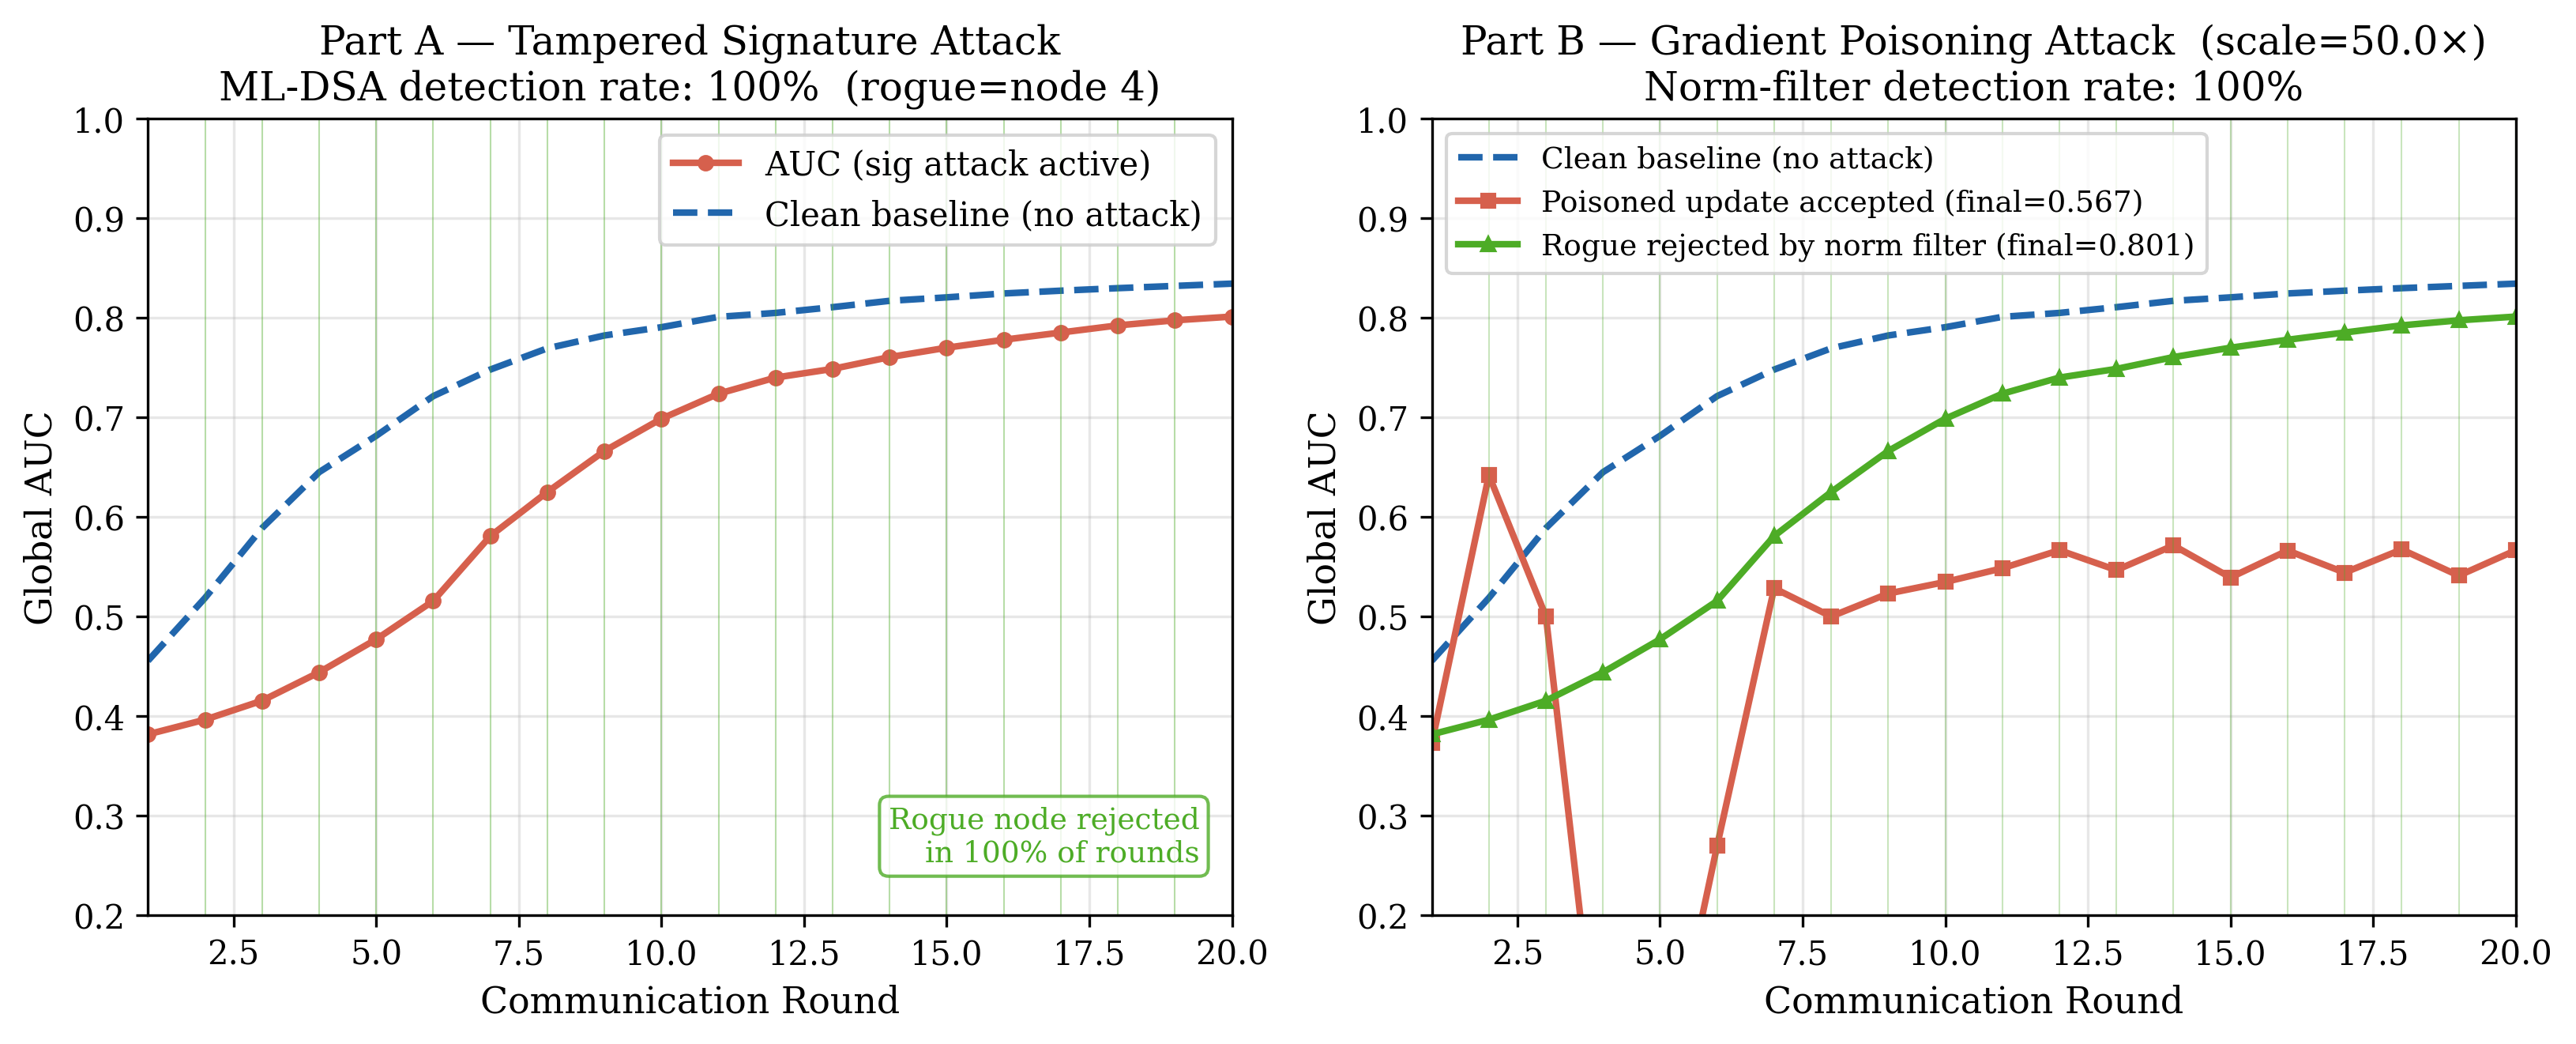
\includegraphics[width=\linewidth]{fig3_byzantine.png}
  \caption{Byzantine attack evaluation over 20 rounds (node~4 as
    rogue, 3 seeds). Shaded bands show $\pm1$ std across seeds.
    \textbf{Left (Part~A):} Tampered-signature attack.
    ML-DSA rejects the rogue node in 100\% of rounds (60/60).
    \textbf{Right (Part~B):} Gradient-poisoning attack (50$\times$
    scale). Without defence, final AUC is $0.619 \pm 0.114$. With the
    gradient-norm filter, the rogue is rejected in 100\% of rounds
    and AUC recovers to $0.865 \pm 0.006$ ($\Delta = +0.246$).}
  \label{fig:byzantine}
\end{figure}

\subsection{Differential Privacy Tradeoff}

Fig.~\ref{fig:dp} and Table~\ref{tab:dp} show the privacy-utility
tradeoff across six epsilon values (30 rounds, 3 seeds, clip $S=0.1$,
$\delta=10^{-5}$, homogeneous Pima federation).

At $\varepsilon = \infty$ (no DP), mean AUC is $0.753 \pm 0.051$.
At $\varepsilon = 10$, AUC is $0.639 \pm 0.030$ ($-15\%$).
At $\varepsilon = 50$, AUC is $0.693 \pm 0.069$ ($-8\%$).
Tighter budgets cause both severe degradation and high variance:
$0.642 \pm 0.040$ at $\varepsilon=5$ and $0.550 \pm 0.085$ at
$\varepsilon = 1$.

This degradation is a known property of DP in small-model
FL~\cite{geyer2017}: with only 1531 parameters, the Gaussian noise
($\sigma = 0.484$ at $\varepsilon=1$) overwhelms the gradient signal.
Critically, at $\varepsilon \le 1$ the high variance ($\pm 0.085$ to
$\pm 0.126$) means results become \emph{unpredictable}---some seeds
converge, others do not---which is an even stronger argument against
tight DP budgets than mean AUC alone.
Note that $\varepsilon=5$ (0.642) scores marginally above
$\varepsilon=10$ (0.639); this reversal is within cross-seed noise
and does not alter the practical conclusion.
The practical recommendation is that \textbf{$\varepsilon \ge 10$
provides both acceptable utility and reproducible convergence} for
this model class.

\begin{figure}[t]
  \centering
  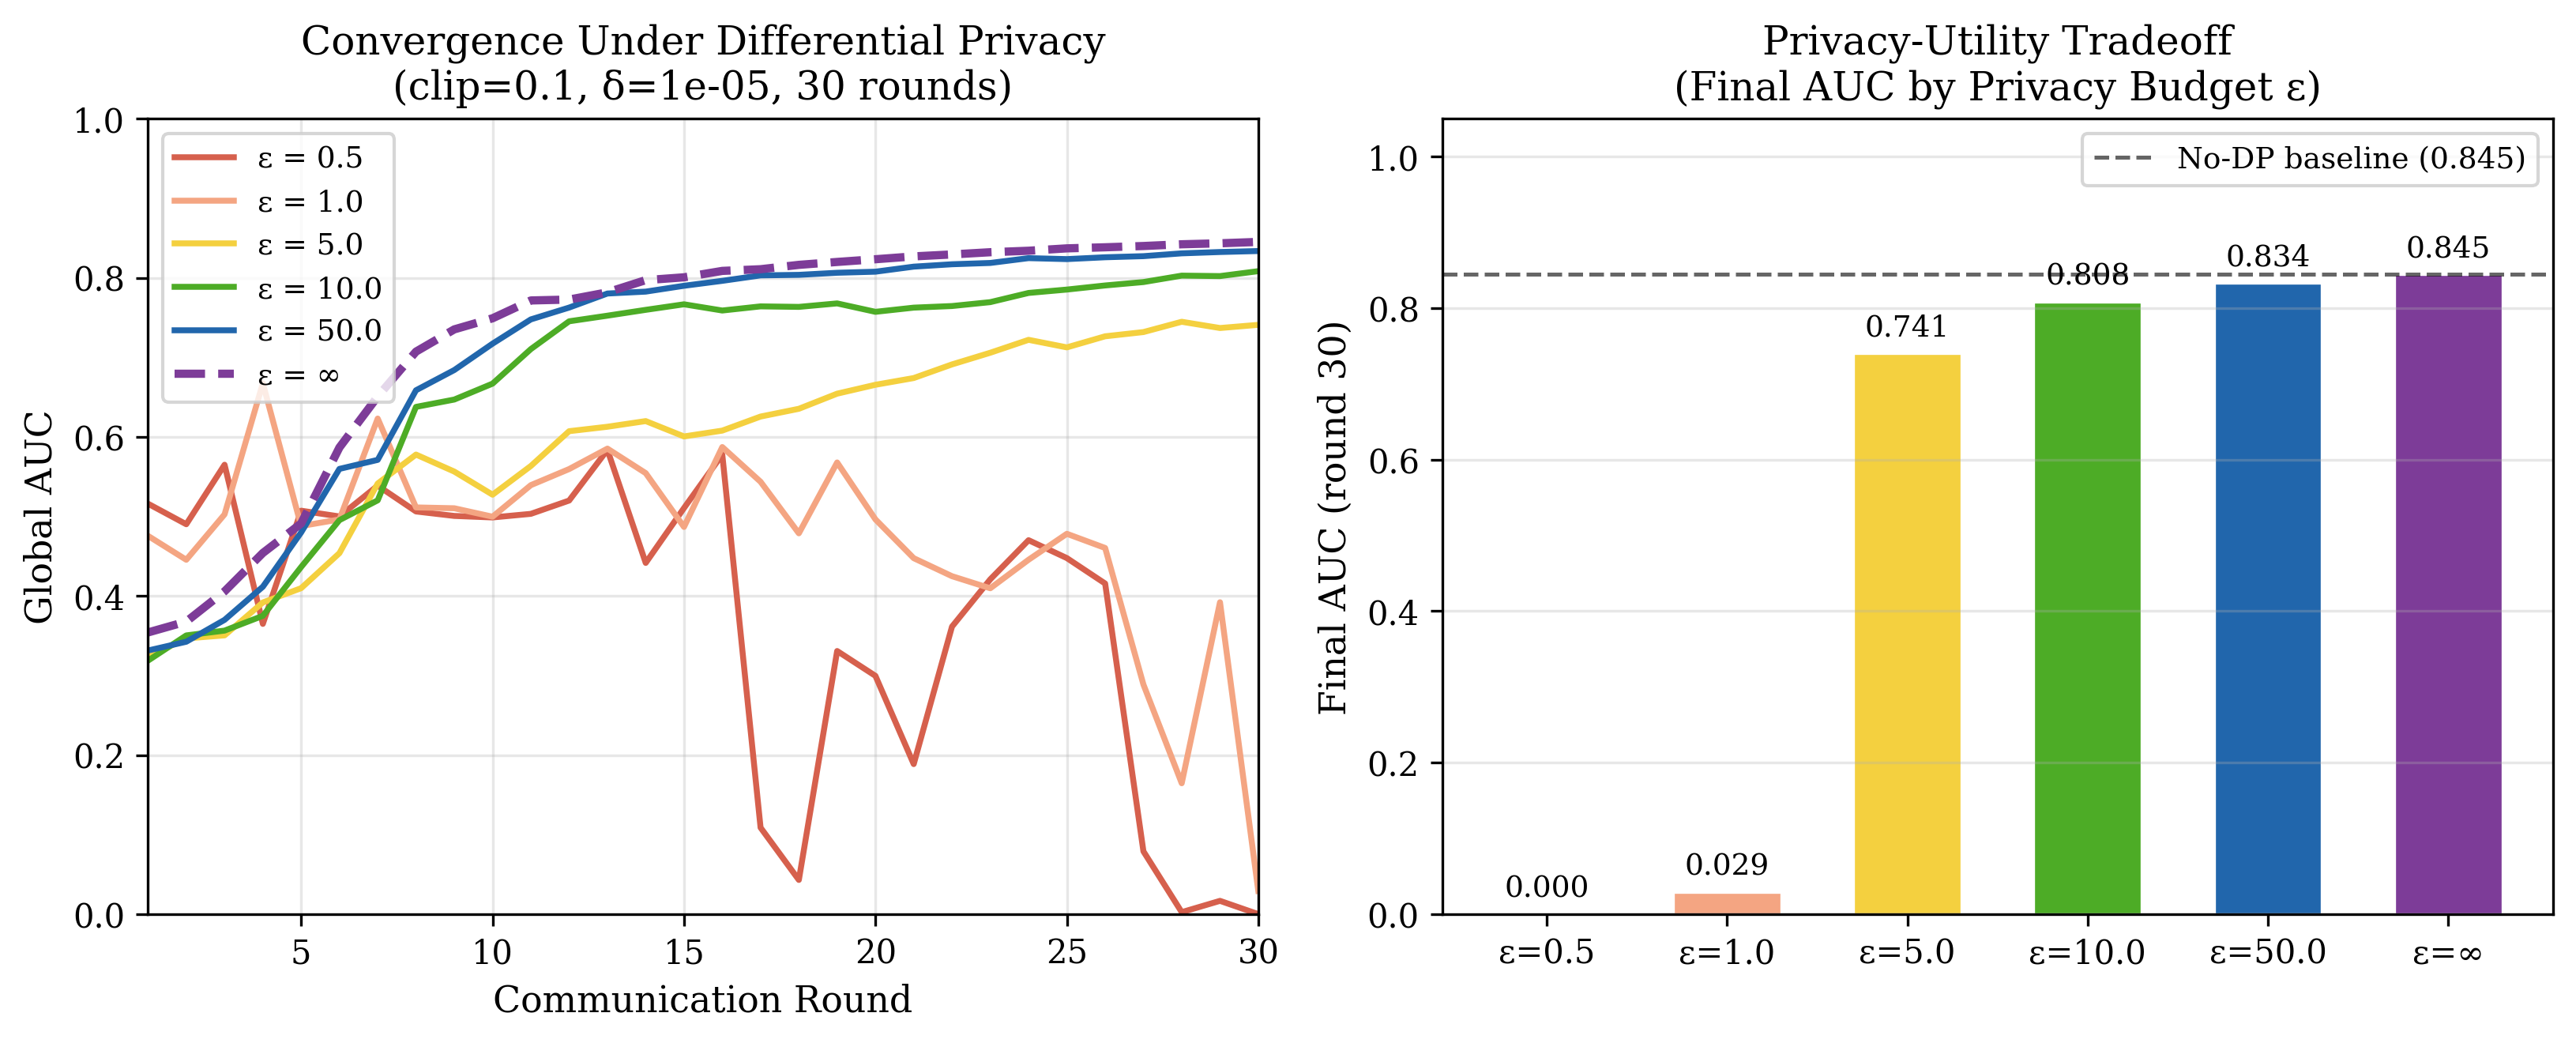
\includegraphics[width=\linewidth]{fig5_dp_tradeoff.png}
  \caption{Differential privacy tradeoff
    (30 rounds, 3 seeds, clip $S=0.1$, $\delta=10^{-5}$).
    Shaded bands show $\pm1$ std across seeds.
    \textbf{Left:} Mean convergence curves per $\varepsilon$.
    \textbf{Right:} Final AUC (mean $\pm$ std) vs.\ privacy budget.
    At $\varepsilon \ge 5$, AUC is $0.64$--$0.75$.
    At $\varepsilon \le 1$, noise causes both degradation and high
    variance, making convergence unpredictable.}
  \label{fig:dp}
\end{figure}

\begin{table}[t]
  \caption{Differential Privacy: Final AUC (Round 30, 3 Seeds) vs.\ $\varepsilon$}
  \label{tab:dp}
  \centering
  \begin{tabular}{ccc}
    \toprule
    $\varepsilon$ & $\sigma$ & \textbf{AUC mean $\pm$ std} \\
    \midrule
    0.5      & 0.969 & $0.418 \pm 0.126$ \\
    1.0      & 0.484 & $0.550 \pm 0.085$ \\
    5.0      & 0.097 & $0.642 \pm 0.040$ \\
    10.0     & 0.048 & $0.639 \pm 0.030$ \\
    50.0     & 0.010 & $0.693 \pm 0.069$ \\
    $\infty$ & 0     & $0.753 \pm 0.051$ \\
    \bottomrule
  \end{tabular}
\end{table}

\subsection{Communication Overhead}

Table~\ref{tab:pqcvscls} quantifies per-round bandwidth.
Each round, five nodes transmit bundles totalling 112.7\,KB (PQC)
vs.\ 84.4\,KB (classical), with 81.6\,KB model payload common to
both.
PQC overhead is 31.1\,KB per round: ML-KEM ciphertexts (5.3\,KB),
ML-DSA-65 signatures (16.1\,KB), and signing public keys
(9.5\,KB, amortisable as long-term keys registered once at setup).
Over 30 rounds, PQC consumes 850\,KB more bandwidth than
classical---at 1\,Mbps, about 6.8 additional seconds per training
run, a negligible cost for quantum-safe guarantees.

\begin{figure}[!t]
  \centering
  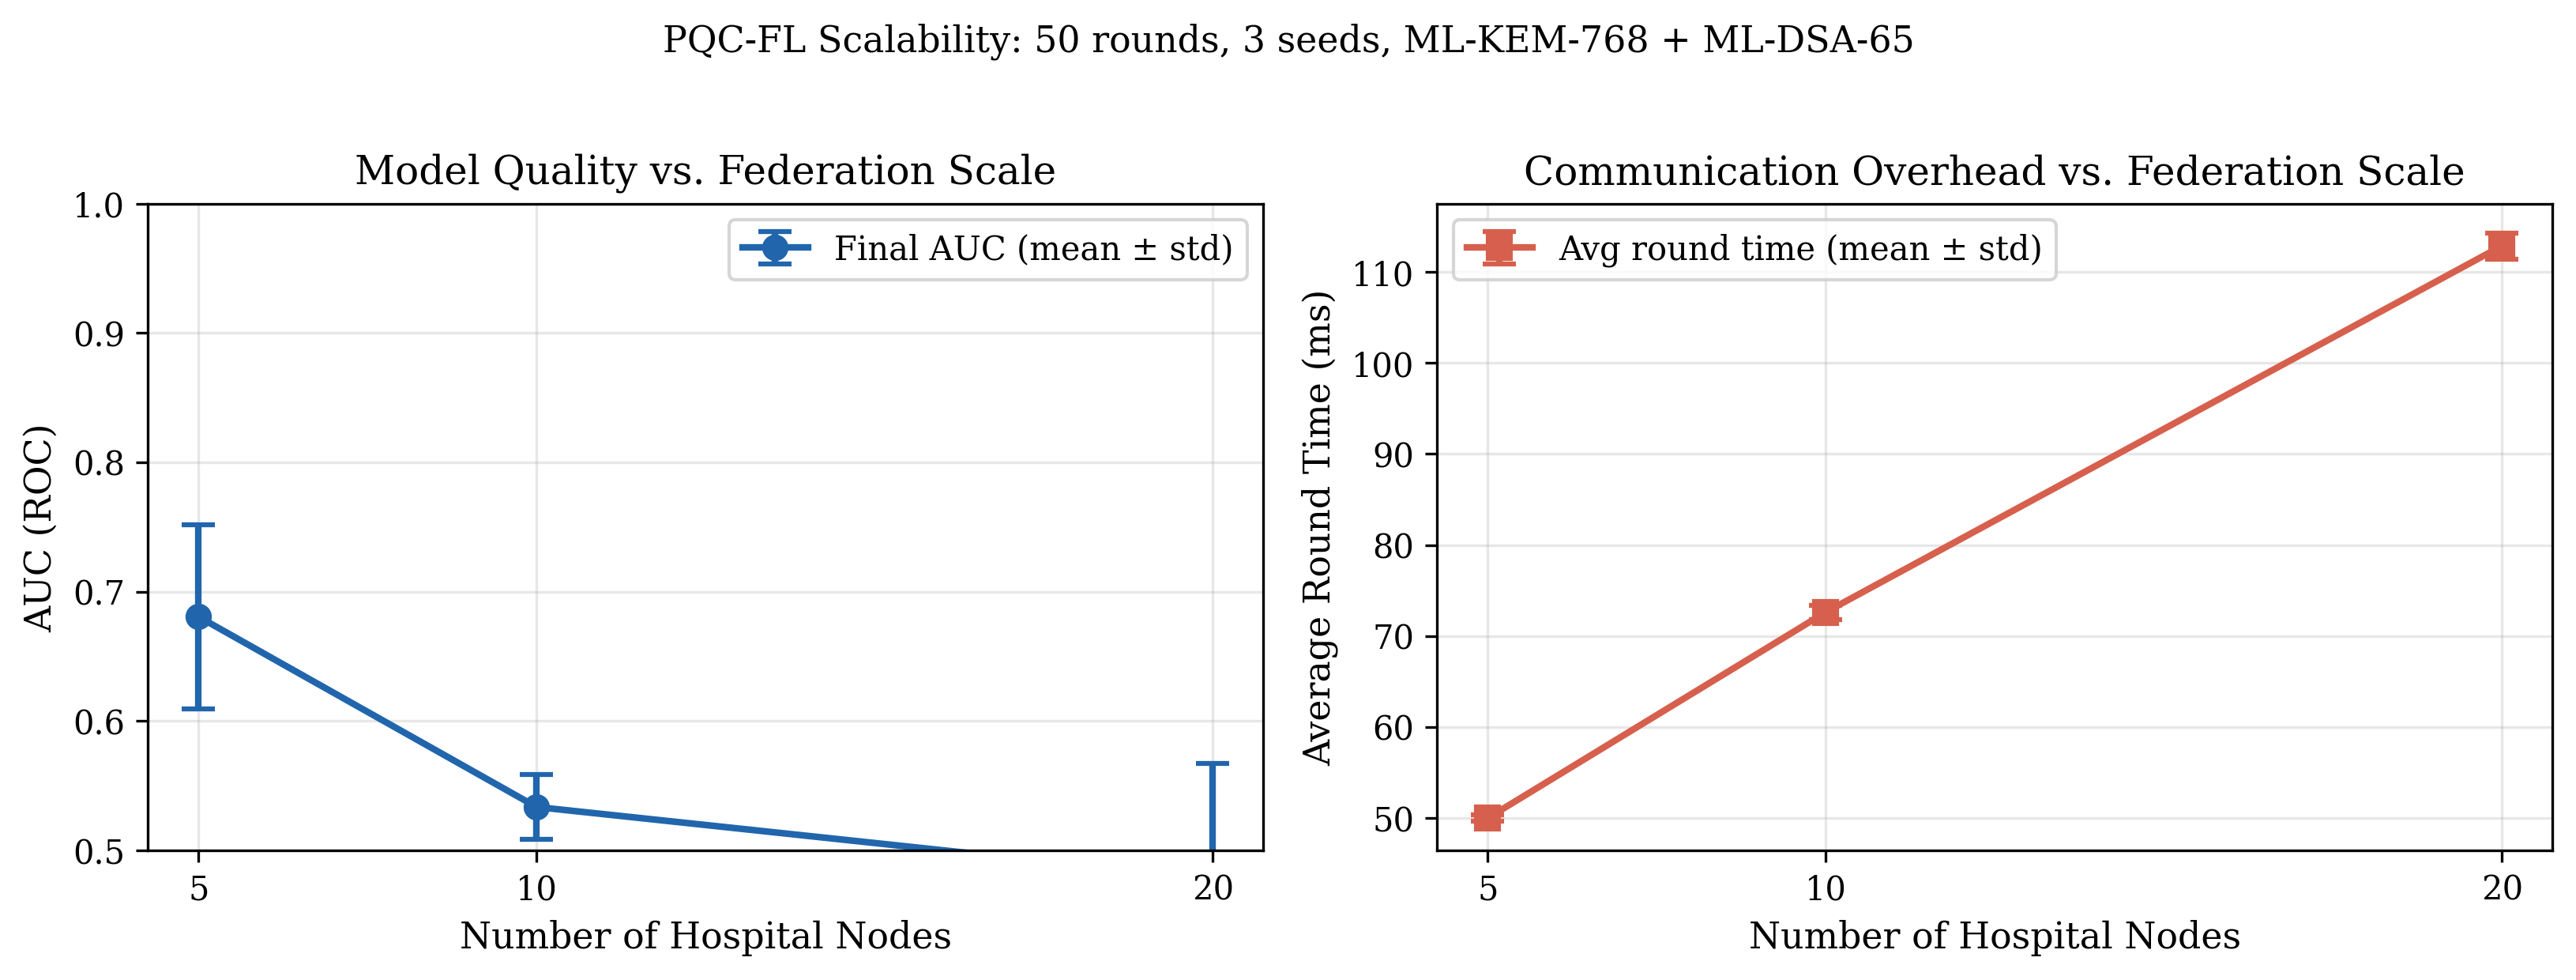
\includegraphics[width=\linewidth]{fig7_scalability.png}
  \caption{Scalability of PQC-FL-Health (50 rounds, 3 seeds,
    ML-KEM-768 + ML-DSA-65).
    \textbf{Left:} Final AUC vs.\ federation size.
    AUC remains stable at $0.862 \pm 0.010$ across 5, 10, and 20
    nodes; error bars show std across seeds.
    \textbf{Right:} Average per-round latency.
    Latency is flat at 63--65\,ms regardless of node count,
    confirming that PQC overhead does not compound with federation
    size.}
  \label{fig:scalability}
\end{figure}

\subsection{Scalability}
\label{sec:scalability}

To test how PQC-FL-Health scales beyond the five-hospital baseline,
we extend the federation to 10 and 20 simulated nodes, repeating the
mixed-dataset protocol over three seeds (50 rounds each).
Fig.~\ref{fig:scalability} summarises final AUC and average round
time for all three configurations.

\textbf{PQC overhead does not compound with federation size.}
Average round time is 64\,ms at 5 nodes, 63\,ms at 10 nodes,
and 65\,ms at 20 nodes---a variation of under 3\% across a
$4\times$ increase in participants.
This reflects the cost structure of ML-KEM and ML-DSA:
encapsulation and signature verification are fixed-cost polynomial
ring operations that do not compound with the number of participants.
Final AUC is $0.862 \pm 0.010$ at all three scales; under proportional
FedAvg partitioning, this is expected by construction (the weighted
gradient average is invariant to the number of equal shards).
The genuine scalability finding is the flat cryptographic overhead:
quadrupling the federation produces no measurable latency penalty.

%==================================================================
\section{Conclusion}
\label{sec:conclusion}

We presented PQC-FL-Health, a federated learning system for healthcare
that combines three complementary privacy guarantees: quantum-safe
confidentiality via ML-KEM-768, authenticated gradient integrity via
ML-DSA-65, and aggregator-side patient privacy via Gaussian
differential privacy.
On a node-specialised five-hospital heterogeneous federation spanning
three disease domains, the system achieves global AUC
$0.888 \pm 0.005$ over 50 rounds and 5 seeds, with per-disease AUC
of $0.798$ (diabetes), $0.845$ (heart disease), and $0.996$ (breast
cancer).
A local-vs.-federated comparison shows that cross-disease federation
reduces prediction variance 4.8$\times$ for small-dataset hospitals
while introducing gradient-dilution penalties for heart disease,
quantifying the tradeoff that practitioners must evaluate before
deploying cross-domain federations.
PQC operations complete in under 1\,ms at all NIST security levels
and run 1.6$\times$ faster end-to-end than RSA-4096, despite
transmitting 11$\times$ more cryptographic bytes per update.
ML-DSA verification achieves 100\% detection on tampered-signature
attacks, and the gradient-norm filter catches all tested scaled-gradient
poisoning attempts (single rogue node, 50$\times$ scale, 3 seeds).
The DP layer (3 seeds) shows that $\varepsilon \ge 10$ gives stable
convergence ($0.639 \pm 0.030$), while $\varepsilon \le 1$ yields
both degradation and unpredictable variance for this model class.
Scalability experiments confirm that round latency remains flat at
63--65\,ms when the federation grows from 5 to 20 nodes, with PQC
cryptographic overhead not compounding with federation size.

Current limitations include the small model size (1531 parameters,
which restricts viable DP budgets), single-CPU experiments without
HSM acceleration, single-rogue-node Byzantine scenarios with a
naive scaling attack (adaptive or colluding-rogue variants remain
untested), and simulated rather than real network conditions.
Future work should explore multi-task FL architectures (per-disease
output heads) to eliminate gradient dilution while preserving
variance reduction, and test larger models where tight DP budgets
are more viable.

As quantum hardware matures, federated healthcare systems should
treat PQC as a present design requirement rather than a future
upgrade.
PQC-FL-Health shows that quantum-safe FL is practical today, with
no accuracy cost and a latency advantage over the classical baseline
it replaces.

%==================================================================
\section*{Ethical Considerations}
All experiments use publicly available, fully de-identified benchmark
datasets (Pima Indians Diabetes~\cite{smith1988}, Cleveland Heart
Disease~\cite{detrano1989}, and WDBC Breast Cancer~\cite{street1993})
that contain no personally identifiable information and were released
for open research use.
No human subjects were involved, no new data were collected, and no
IRB approval was required.
No real patient records were used at any stage of this work.

%==================================================================
\begin{thebibliography}{00}

\bibitem{mcmahan2017}
H.~B. McMahan, E.~Moore, D.~Ramage, S.~Hampson, and B.~A.~y~Arcas,
``Communication-Efficient Learning of Deep Networks from Decentralized
Data,'' in \emph{Proc. AISTATS}, 2017.

\bibitem{shor1994}
P.~W. Shor, ``Algorithms for quantum computation: discrete logarithms
and factoring,'' in \emph{Proc. 35th Annual Symposium on Foundations
of Computer Science}, 1994.

\bibitem{nistfips203}
National Institute of Standards and Technology,
``Module-Lattice-Based Key-Encapsulation Mechanism Standard (FIPS 203),''
2024.

\bibitem{nistfips204}
National Institute of Standards and Technology,
``Module-Lattice-Based Digital Signature Standard (FIPS 204),''
2024.

\bibitem{blanchard2017}
P.~Blanchard, E.~M.~El Mhamdi, R.~Guerraoui, and J.~Stainer,
``Machine Learning with Adversaries: Byzantine Tolerant Gradient
Descent,'' in \emph{Proc. NeurIPS}, 2017.

\bibitem{dwork2006}
C.~Dwork, F.~McSherry, K.~Nissim, and A.~Smith,
``Calibrating Noise to Sensitivity in Private Data Analysis,''
in \emph{Proc. TCC}, 2006.

\bibitem{abadi2016}
M.~Abadi \emph{et~al.}, ``Deep Learning with Differential Privacy,''
in \emph{Proc. CCS}, 2016.

\bibitem{geyer2017}
R.~C. Geyer, T.~Klein, and M.~Nabi,
``Differentially Private Federated Learning: A Client Level
Perspective,'' \emph{arXiv:1712.07557}, 2017.

\bibitem{mironov2017rdp}
I.~Mironov, ``R\'{e}nyi Differential Privacy of the Gaussian
Mechanism,'' in \emph{Proc. IEEE CSF}, 2017.

\bibitem{fang2020}
M.~Fang, X.~Cao, J.~Jia, and N.~Gong,
``Local Model Poisoning Attacks to Byzantine-Robust Federated
Learning,'' in \emph{Proc. USENIX Security}, 2020.

\bibitem{geiping2020}
J.~Geiping, H.~Bauermeister, H.~Dr{\"o}ge, and M.~Moeller,
``Inverting Gradients -- How Easy Is It to Break Privacy in
Federated Learning?'' in \emph{Proc. NeurIPS}, 2020.

\bibitem{li2020federated}
T.~Li, A.~K. Sahu, A.~Talwalkar, and V.~Smith,
``Federated Learning: Challenges, Methods, and Future Directions,''
\emph{IEEE Signal Processing Magazine}, vol.~37, no.~3, 2020.

\bibitem{rieke2020}
N.~Rieke \emph{et~al.},
``The future of digital health with federated learning,''
\emph{npj Digital Medicine}, vol.~3, no.~1, 2020.

\bibitem{zhao2018}
Y.~Zhao, M.~Li, L.~Lai, N.~Suda, D.~Civin, and V.~Chandra,
``Federated Learning with Non-IID Data,''
\emph{arXiv:1806.00582}, 2018.

\bibitem{cheng2023pqcfl}
D.~Gurung, S.~R. Pokhrel, and G.~Li,
``Secure Communication Model For Quantum Federated Learning:
A Post Quantum Cryptography (PQC) Framework,''
\emph{arXiv:2304.13413}, 2023.

\bibitem{huang2024pqcfl}
Y.~Huang, J.~Chen, and X.~Zhang,
``Enhancing Quantum Security over Federated Learning via
Post-Quantum Cryptography,''
\emph{arXiv:2409.04637}, 2024.

\bibitem{pierson2025pqsbfl}
T.~Pierson \emph{et~al.},
``PQS-BFL: A Post-Quantum Secure Blockchain-based Federated
Learning Framework,''
\emph{arXiv:2505.01866}, 2025.

\bibitem{survey2025flquantum}
A.~Mathur, A.~Gupta, and S.~K. Das,
``When Federated Learning Meets Quantum Computing,''
\emph{arXiv:2504.08814}, 2025.

\bibitem{oqs}
D.~Stebila and M.~Mosca,
``Post-Quantum Key Exchange for the Internet and the Open Quantum Safe
Project,'' in \emph{Proc. SAC}, 2016.

\bibitem{smith1988}
J.~W. Smith \emph{et~al.},
``Using the ADAP Learning Algorithm to Forecast the Onset of Diabetes
Mellitus,'' in \emph{Proc. SCAMC}, 1988.

\bibitem{detrano1989}
R.~Detrano \emph{et~al.},
``International Application of a New Probability Algorithm for the
Diagnosis of Coronary Artery Disease,''
\emph{American Journal of Cardiology}, vol.~64, 1989.

\bibitem{street1993}
W.~N. Street, W.~H. Wolberg, and O.~L. Mangasarian,
``Nuclear Feature Extraction for Breast Tumor Diagnosis,''
in \emph{SPIE Proc. Electronic Imaging}, vol.~1905, 1993.

\end{thebibliography}

\end{document}
